\section{Terminology}
Queueing theory studies systems and processes in terms of three key concepts:
\begin{itemize}
\item \textbf{customers} are the units of work that the system serves -- a customer can be a real person, or it can be whatever the system is supposed to process and complete: a web request, a database query, a part to be milled by a machine, etc.;
\item \textbf{servers} are the objects that do the processing work -- a server might be the cashier at the grocery store, a web server, a database server, a milling machine, etc., and 
\item \textbf{queues} are where the units of work wait if the server is busy and can not start the work as they arrive -- a queue may be a physical line, reside in memory, etc. 
\end{itemize}
In order to describe queues, we must first know and understand some useful probability distributions, as well as input and output processes.
\subsection{Exponential and Poisson Probability Distributions}
The \textbf{Poisson} and \textbf{exponential} distributions play a prominent role in queuing theory. The Poisson distribution counts the number of discrete events occurring in a fixed time period; it is closely connected to the exponential distribution, which (among other applications) measures the time between arrivals of the events. The Poisson distribution is a discrete distribution; the random variable can only take non-negative integer values. The exponential distribution can take any (nonnegative) real value.
\newl Consider the problem of determining the probability of $n$ arrivals being observed during a time interval of length $t$, where the following assumptions are made:
\begin{itemize}
\item the probability that an arrival is observed during a small time interval (say of length $\nu$) is proportional to the length of interval; let the proportionality constant be $\lambda$, so that the probability is $\lambda\nu$;
\item the probability of two or more arrivals in a small interval is zero, and 
\item the number of arrivals in any time interval is independent of the number in non-overlapping time interval (for example, the number of arrivals occurring between times 5 and 25 does not provide information about the number of arrivals occurring between times 30 and 50).
\end{itemize}
\begin{figure}[!t]
\centering
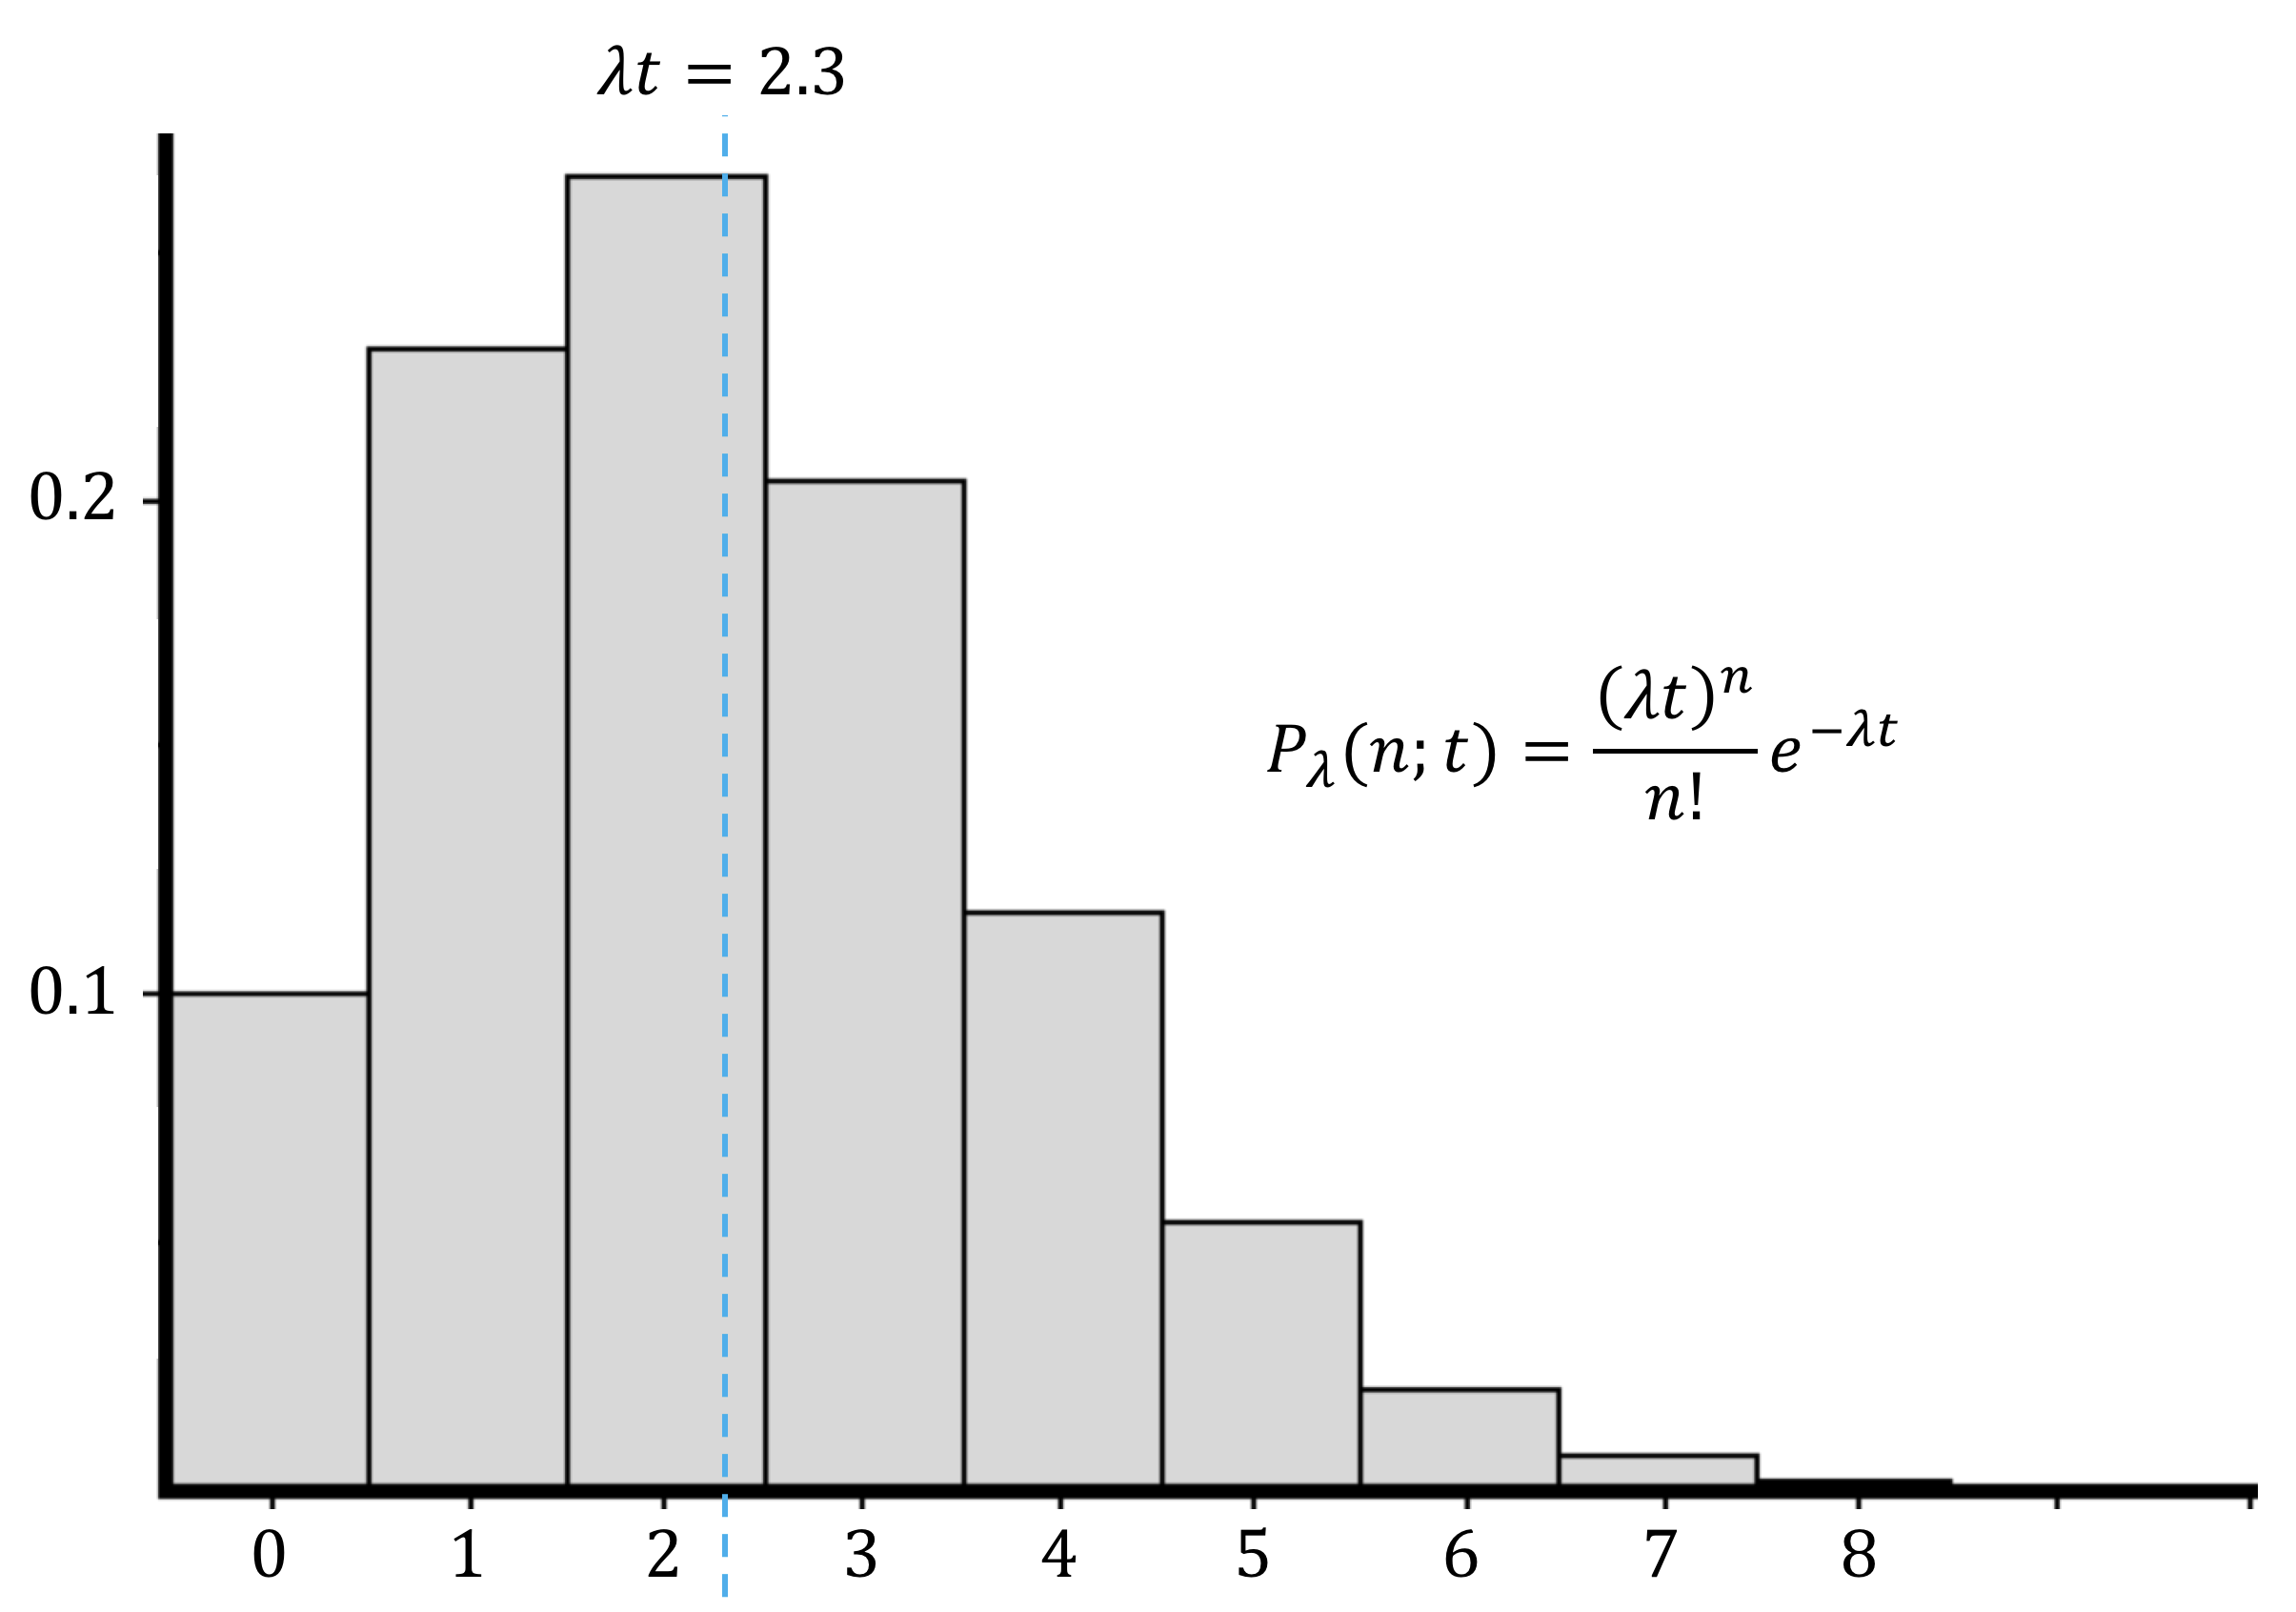
\includegraphics[height=0.25\textheight]{Images/poisson.png}
\centering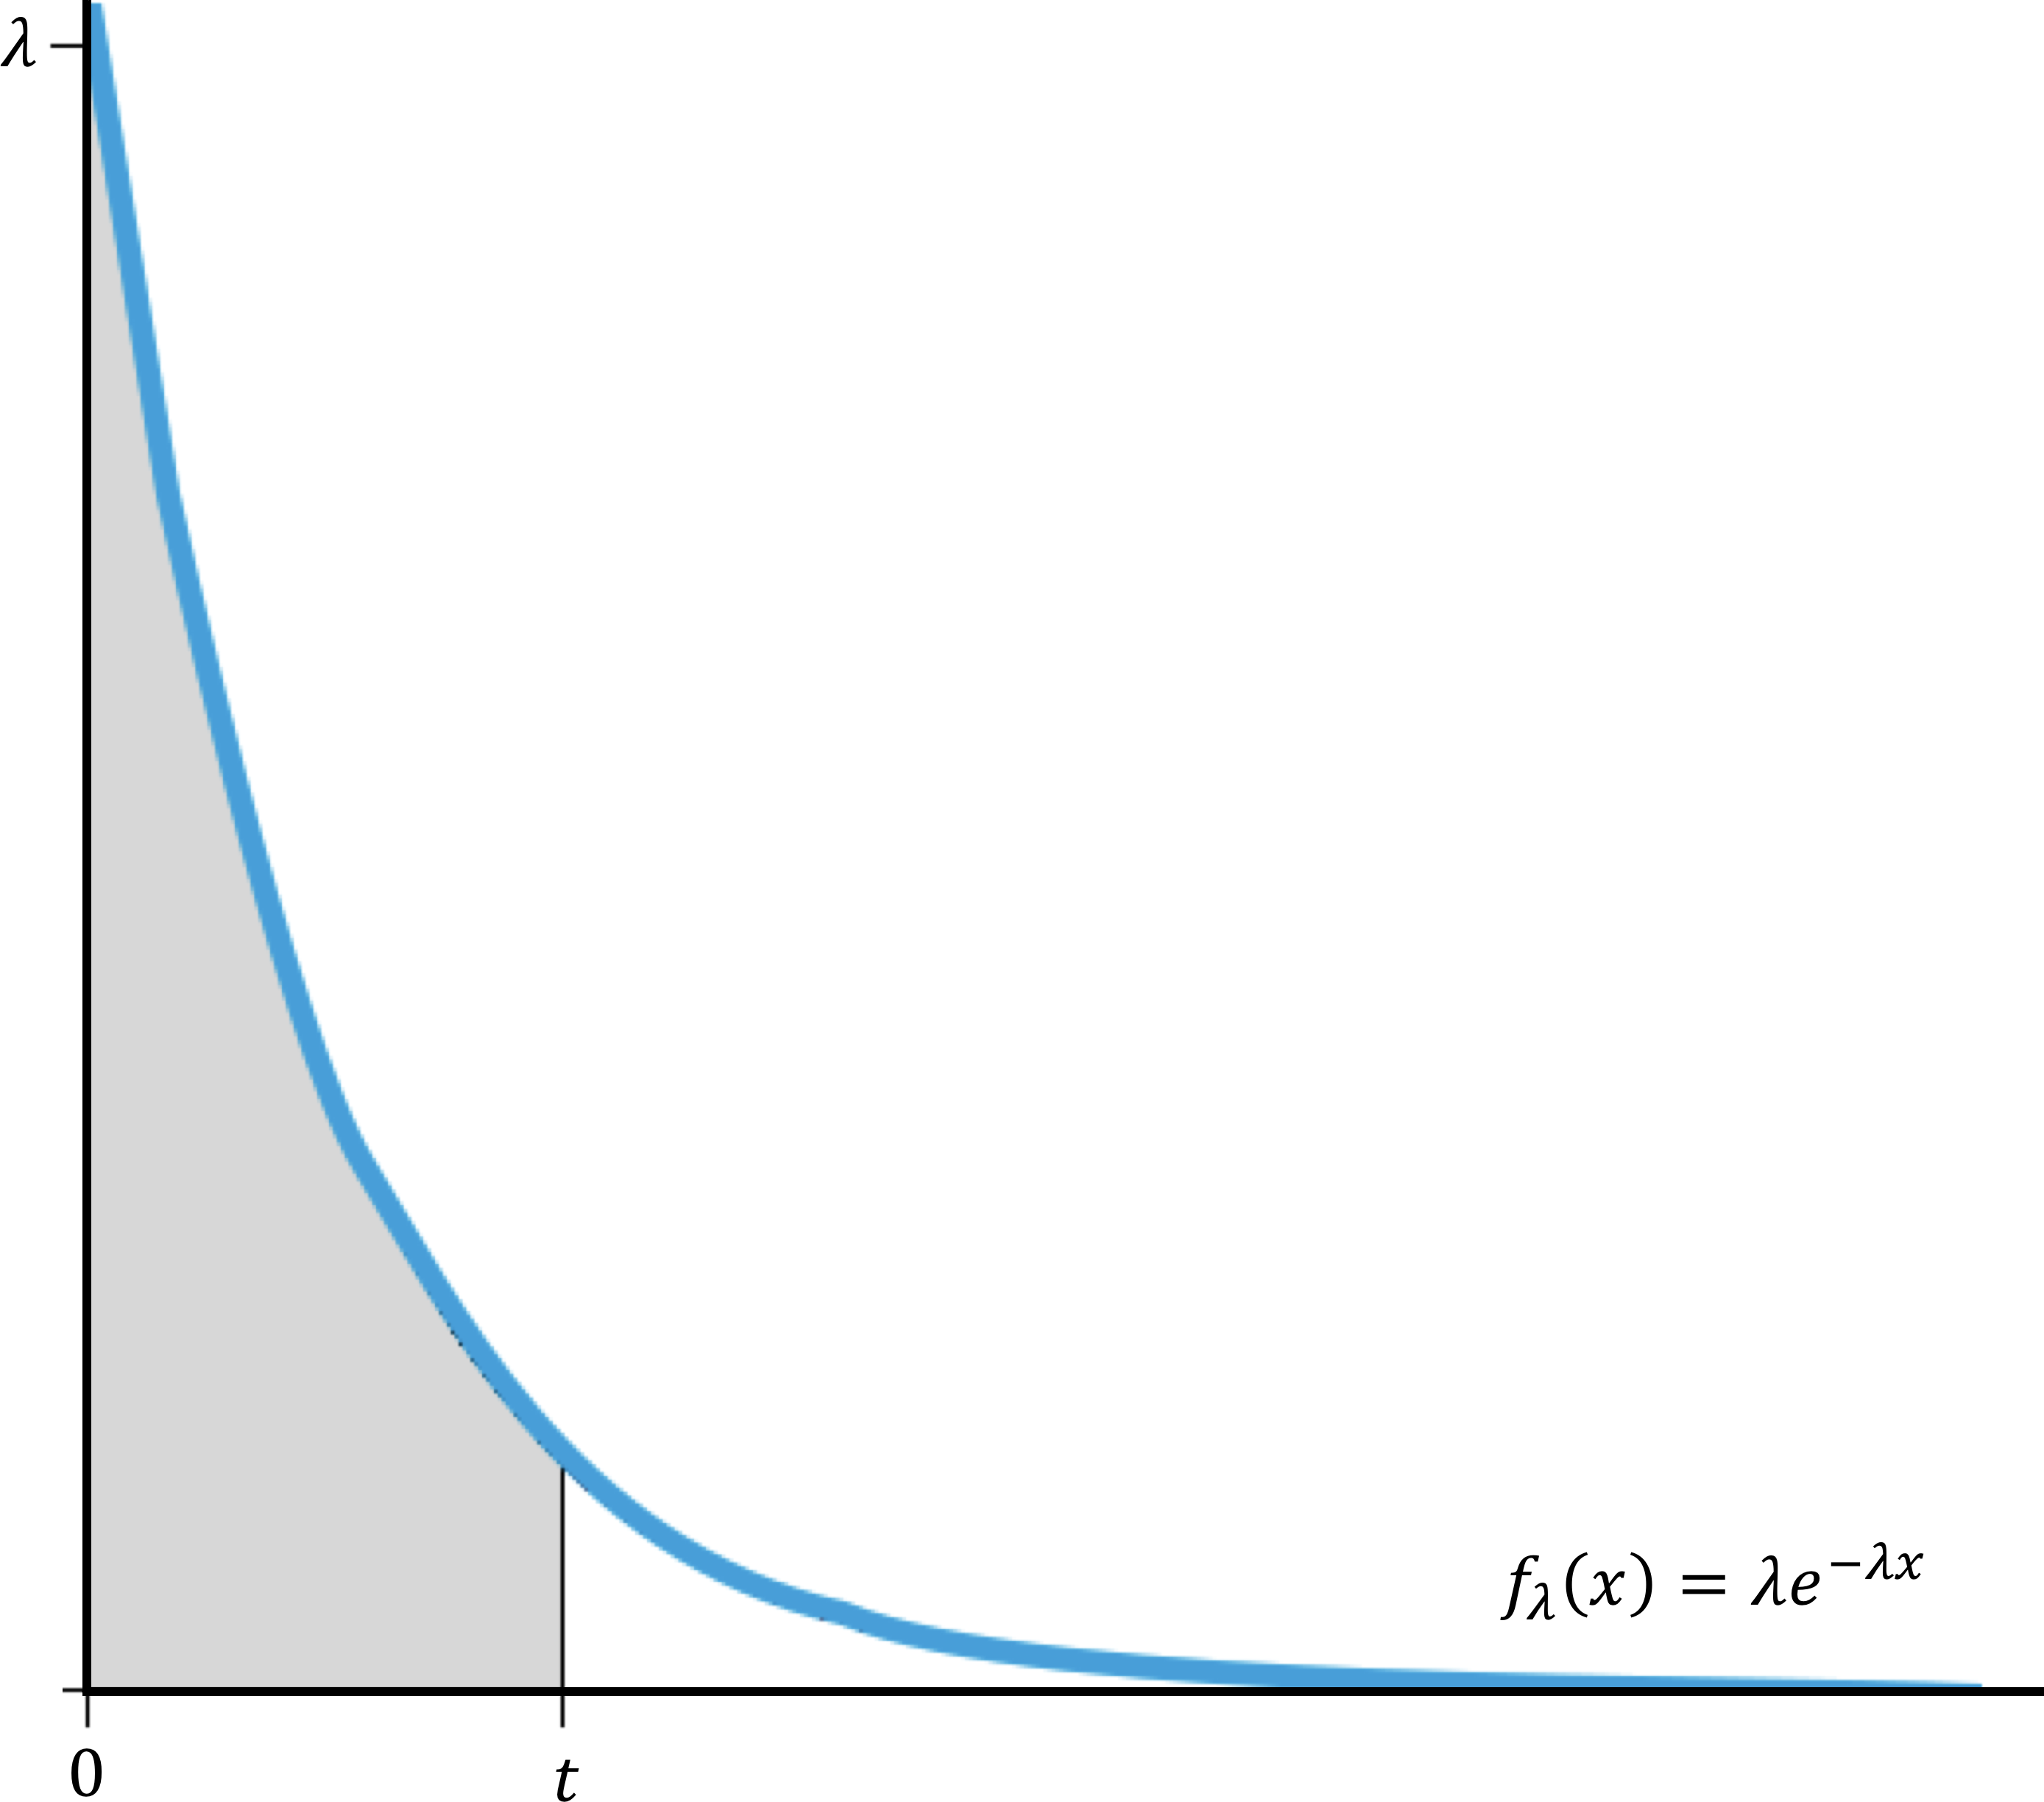
\includegraphics[height=0.25\textheight]{Images/exp.png}
\caption{\small Poisson (with $\lambda t=2.3$) and exponential distributions (with parameter $\lambda$). The shaded area (bottom image) represents the probability that a customer will wait up to the length of the time interval $t$.}\label{fig:dist1}\hrule
\end{figure}
Now, let $P(n;t)$ be the probability of observing $n$ arrivals in a time interval of length $t$.
Then, for some $\lambda>0$, 
$$ P_{\lambda}(n; t) = \frac{(\lambda t)^n}{n!} e^{-\lambda t}, \ n=0,1,2,\cdots$$
is the p.m.f. of the \textbf{Poisson distribution} for the discrete random variable $n$ -- the number of arrivals -- for a given length of time interval $t$ (see Figure~\ref{fig:dist1}). In a queueing system, such arrivals are referred to as \textbf{Poisson arrivals}. \newl The time between successive arrivals is called the \textbf{inter-arrival time}. If the number of arrivals in a given time interval follows a Poisson distribution with parameter $\lambda t$, the inter-arrival times follow an exponential distribution with p.d.f. 
$$ f_{\lambda}(t) = \lambda e^{-\lambda t}, \ \textrm{for }t>0,$$ and the probability $P(W\leq t)$ that a customer's waiting time $W$ is smaller than the length of the time interval $t$ is  
$$P(W\leq t) = 1 - e^{-\lambda t}\quad \textrm{(see Figure~\ref{fig:dist1})}.$$
In general, if the arrival rate is \textbf{stationary}, if \textbf{bulk} arrivals (two or more simultaneous arrivals) cannot occur, and if past arrivals do not affect future arrivals, then inter-arrival times follow an exponential distribution with parameter~$\lambda$, and the number of arrivals in any interval of length $t$ is Poisson with parameter $\lambda t$. \newl One of the most attractive features of the exponential distribution relating to inter-arrival times is that it is \textbf{memoryless} --  if a random variable $X$ follows an exponential distribution, then for all non-negative values of $t$ and $h$,
\begin{equation}
P(X \geq t + h|X \geq t) = P(X \geq h). 
\label{eq:1}
\end{equation}
No other density function satisfies $(\ref{eq:1})$ \cite{QS_R}. The memoryless property of the exponential distribution is important because it implies that the probability distribution of the time until the next arrival is independent of the time since the last arrival -- imagine if that was the case when waiting for public transportation! \par For instance, if we know that at least $t$ time units have elapsed since the last arrival, then the distribution of the time $h$ until the next arrival is independent of $t$. If $h=4$, say, then $(\ref{eq:1})$ yields 
$$ P(X>9|X>5)= P(X>7|X>3) = P(X>4).$$

\subsection{Erlang Distribution}
The exponential distribution is not always an appropriate model of inter-arrival times, however (perhaps the process should not be memoryless, say). A common alternative is to use the \textbf{Erlang} distribution $\mathcal{E}(R,k)$, a continuous random variable with \textbf{rate} and \textbf{shape} parameters $R>0$ and $k\in \mathbb{Z}^+$, respectively, whose p.d.f. is  
$$ f_{R,k}(t) = \frac{R (Rt)^{k-1} e^{-Rt}}{(k-1)!},\ t\geq 0.$$
When $k=1$, the Erlang distribution reduces to an exponential distribution with parameter $R$. It can be shown that if $X\sim \mathcal{E}(k\lambda,k)$, then  $X\sim X_{1}+X_{2}+\cdots+X_{k},$ where each $X_{i}$ is an independent exponential random variable with parameter $k \lambda$. \newl When we model the inter-arrival process as an Erlang distribution $\mathcal{E}(k\lambda,k)$, we are really saying that it is equivalent to customers going through $k$ \textbf{phases} (each of which is memoryless) before being served. For this reason, the shape parameter is often referred to as the number of phases of the Erlang distribution \cite{QS_N}.
\subsection{Input/Arrival Process}
The input process is usually called the \textbf{arrival process}. Arrivals are called \textbf{customers}. In the models under consideration, we assume that arrivals cannot be simultaneous (this might be unrealistic when modeling arrivals at a restaurant, say). If simultaneous arrivals are possible (in theory and/or in practice), we say that \textbf{bulk arrivals are allowed}. 
\par Usually, we assume that the arrival process is \textbf{unaffected by the number of customers} in the system. In the context of a bank, this would imply that whether there are 500 or 5 people at the bank, the process governing arrivals remains unchanged.  
\newl There are two common situations in which the arrival process may depend on the number of customers present. The first occurs when arrivals are drawn from a small population -- the so-called \textbf{finite source models} -- if all members of the population are already in the system, there cannot be another arrival!\par Another such situation arises when the rate at which customers arrive at the facility decreases when the facility becomes too crowded. For example, when customers see that a restaurant's parking lot is full, they might very well decide to go to another restaurant or forego eating out altogether. If a customer arrives but fails to enter the system, we say that the customer has \textbf{balked}.
\subsection{Output/Service Process}
To describe the output process (often called the \textbf{service process}) of a queuing system, we usually specify a probability distribution -- the \textbf{service time distribution} -- which governs the customers' service time. \par In most cases, we assume that the service time distribution is independent of the number of customers present in the system. This implies, for example, that the server does not work faster when more customers are present. \newl We can distinguish two types of servers: \textbf{in parallel} and \textbf{in series}. Servers are in parallel if they all provide the same type of service and a customer only needs to pass through one of them to complete their service. For example, the tellers in a bank are usually arranged in parallel; typically, customers only need to be serviced by one teller, and any teller can perform the desired service. \par Servers are in series if a customer must pass through several servers before their service is complete. An assembly line is an example of such a queuing system.
\newl 
Input and output processes occur in a variety of situations:
\begin{itemize}
\item \textbf{situation:} purchasing Blue Jays tickets at the Rogers Centre\\ \textit{input:} baseball fans arrive at the ticket office\\ \textit{output:} tellers serve the baseball fans;
\item \textbf{situation:} pizza parlour \\ \textit{input:} requests for pizza delivery are received; \\\textit{output}: pizza parlour prepares and bakes pizzas, and sends them to be delivered; 
\item \textbf{situation:} government service centre\\ \textit{input}: citizen/residents enter the service centre \\ \textit{output:} receptionist assigns them to a specific queue based on their needs\\
\textcolor{white}{.}\qquad \textit{input:} citizen/residents enter a specific queue\\ \textcolor{white}{.}\qquad based on their needs \\ \textcolor{white}{.}\qquad \textit{output:} public servant addresses their needs;
\item \textbf{situation:} hospital blood bank\\ \textit{input:} pints of blood arrive\\ \textit{output:} patients use up pints of blood;
\item \textbf{situation:} garage\\ \textit{input:} cars break down and are sent to the garage for repairs\\ \textit{output:} cars are repaired by mechanics and sent back on the streets.
\end{itemize}
The relevant computations are fairly easy to execute, as the following examples demonstrate.
\begin{Example} On average, 4.6 customers enter a coffee shop each hour. If the arrivals follow a Poisson process, the probability that at most two customers will enter in a 30 minute period is \begin{align*}P_{\lambda=4.6}&(n\leq 2;t=0.5)=P_{4.6}(0,0.5)+P_{4.6}(1,0.5)+P_{4.6}(2,0.5) \\ &=e^{-4.6\cdot 0.5}\left[\frac{(4.6\cdot 0.5)^0}{0!}+\frac{(4.6\cdot 0.5)^1}{1!}+\frac{(4.6\cdot 0.5)^2}{2!}\right] \\ &\approx 0.5960; \end{align*} the corresponding Poisson distribution is shown in Figure~\ref{fig:dist1}.
\end{Example}
\begin{Example}
 In a fast food restaurant, a cashier serves on average 9 customers in a one-hour time period. If the service time follows an exponential distribution, $77.7\%$ and $1.1\%$ of customers will be served in 10 minutes or less, and after 30 minutes, respectively. Indeed, \begin{align*}P(W\leq 10/60)&=1-e^{-9 \cdot 10/60} \approx 0.7769\\ P(W>30/60)&=e^{-9\cdot 30/60}\approx 0.0111.\end{align*}
\end{Example}

\subsection{Queue Discipline}
To describe a queuing system completely, we must also describe the \textbf{queue discipline} and the manner in which customers \textbf{join lines}. The queue discipline describes the method used to determine the order in which customers are served: 
\begin{itemize}
\item the most common queue discipline is the \textbf{first come, first served} (FCFS) discipline, in which customers are served in the order of their arrival, as one would expect to see in an Ottawa coffee shop;
\item under the \textbf{last come, first served} (LCFS) discipline, the most recent arrivals are the first to enter service; for example, if we consider exiting from an elevator to be the service, then a crowded elevator illustrates such a discipline;
\item sometimes the order in which customers arrive has no effect on the order in which they are served; this would be the case if the next customer to enter service is randomly chosen from those customers waiting for service, a situation referred to as \textbf{service in random order} (SIRO) discipline; when callers to an inter-city bus company are put on hold, the luck of the draw often determines which caller will next be serviced by an operator, 
\item finally, \textbf{priority} discipline classifies each arrival into one of several categories, each of which is assigned a priority level (a \textbf{triage} process); within each priority level, customers enter the queue on a FCFS basis; such a discipline is often used in emergency rooms to determine the order in which customers receive treatment, and in copying and computer time-sharing facilities, where priority is usually given to jobs with shorter processing times.
\end{itemize}

\subsection{Method Used by Arrivals to Join Queue}
Another important factor for the behaviour of the queuing system is the \textbf{method} used by customers to determine which line to join. For example, in some banks, customers must join a single line, but in other banks, customers may choose the line they want to join. \par  When there are several lines, customers often join the shortest line. Unfortunately, in many situations (such as at the supermarket), it is difficult to define the shortest line. If there are several lines at a queuing facility, it is important to know whether or not customers are allowed to \textbf{switch}, or jockey, between lines. In most queuing systems with multiple lines, jockeying is permitted, but jockeying at a custom inspection booth would not be recommended, for instance. 

